\documentclass{article}
\usepackage[utf8]{inputenc}
\usepackage{mathtools}
\usepackage{microtype}
\usepackage{silence}
\usepackage{amsmath}
\usepackage{caption,subcaption}
\usepackage{graphicx}
\usepackage{babel,blindtext}
\usepackage[superscript,biblabel]{cite}
\usepackage{framed}
\usepackage{wrapfig}
\usepackage{setspace}
%\linespread{1.7}
\onehalfspacing
\usepackage{lineno}
\FrameSep2pt
\usepackage[margin=1in]{geometry}
\usepackage{ulem}
\usepackage{tgpagella}
\usepackage{xparse}

\NewDocumentCommand{\evalat}{sO{\big}mm}{%
  \IfBooleanTF{#1}
   {\mleft. #3 \mright|_{#4}}
   {#3#2|_{#4}}%
}

\title{Host phenology can select for multiple stable parasite virulence strategies}
%\author{hannelore.macdonald}
\date{}

\begin{document}

\maketitle

\section*{Abstract}
Host phenology is an important driver of parasite transmission and evolution. In a seasonal environment, monocyclic, obligate-killer parasites evolve optimal virulence strategies such that all parasite progeny are released near the end of the host season to limit parasite progeny death in the environment. Host seasonality could also select for higher virulence strategies in polycyclic parasites that can complete several generations within the host activity period. We develop a mathematical model of a disease system with seasonal host activity to study the evolutionary consequences of host phenology on polycyclic, obligate-killer parasite virulence strategies. Seasonal host activity patterns create multiple, evolutionary stable virulence strategies separated by less-fit strategies (evolutionary repellors). The evolutionary stable strategy (ESS) that evolves in each system is a function of the virulence strategy of the parasite introduced into the system. The trait value of the optimal virulence strategies is determined by two aspects of host phenology: the duration of the host activity period and the distribution in the time at which hosts first become active within each season. Longer host activity periods and more synchronous host emergence drive both evolutionary stable virulence strategies towards lower virulence. The results demonstrate that host phenology can, in theory, maintain diversity in virulence strategies among isolated geographic locations.




\section*{Introduction}
Classic ecological theory predicts that seasonality creates niche space when species compete for a shared resource. In an equilibrial environment, k-selected species mature slowly but are efficient at collecting resources as adults and outcompete r-selected species who mature quickly but are poor competitors for resources\cite{tilman2020resource}. Fluctuating resources in seasonal environments create niche space such that k-selected species who are better competitors when resources are scarce, can coexist with r-selected species, who reproduce quickly when density is low but resources are abundant\cite{koch1974competitive,armstrong1980competitive,litchman2001competition,klausmeier2008floquet}. While its well established that a vast diversity of parasite strategies exist in nature, the evidence for whether seasonality broadly impacts parasite diversity remains equivocal.

The impact of seasonality on the diversity of several traits important for parasite fitness have been studied. 
One of the best examples of seasonality driving parasite diversity comes from work that considered a trade-off between within-season transmission and between-season survival\cite{hamelin2011seasonality}. This study showed that seasonal host absence can drive evolutionary branching such that parasites specialized on initiating new infections within the season coexist with parasites specialized on between-season survival. However a study on a similar system governed by the same trade-off failed to find evidence that seasonality can drive branching\cite{van2010periodicity}. Seasonal host reproduction has also been shown to drive covert/overt parasite infection strategies towards multiple evolutionary attractors\cite{sorrell2009evolution}. Other traits, such as virulence, have not been driven towards evolutionary branching by seasonality\cite{donnelly2013seasonality}.

%The timing of seasonal host activity, or host phenology, drives the timing and prevalence of transmission opportunities for parasites\cite{Biere1996,Altizer2006,Hamer2012,Gethings2015,Ogden2018,Martinez2018,McDevitt-Galles2020,MacDonald2020}. Host phenology also impacts parasite evolution with the majority of research focused on the evolution of parasite virulence\cite{king2009evolution,sorrell2009evolution,van2011periodic,donnelly2013seasonality}. Whether seasonality could drive parasite diversity by selecting for distinct parasite virulence strategies is unknown.  

Recent work on a disease system with a monocyclic (parasites that complete one generation per season), obligate host-killer parasite demonstrated that seasonal host absence drives the evolution of lower virulence strategies that release new parasites near the end of the host's season. This work further explored how the timing of seasonal host activity, or host phenology, impacts parasite evolution and demonstrated that the exact host phenological pattern determines the virulence level that maximizes parasite fitness. Seasonal parasites are often polycyclic and complete more than one generation per season. Its reasonable to expect that host phenology could have different impacts on polycyclic parasites as compared to monocylic parasites and that these different selection pressures could generate diversity. 

Here we investigate the impact of host phenology on the virulence evolution of an obligate-killer parasite with no constraints on the number of infection cycles it can complete per season. We extend a mathematical model that tracks the dynamics of a monocyclic parasite that infects a seasonally available host species to study the impacts of seasonal host activity on polycyclic parasites. We demonstrate that seasonality drives either low virulence or high virulence to evolve for a parasite population starting from moderate virulence, \textit{i.e.} seasonality can drive bistability in virulence strategies. Further, host season length and the synchronicity at which hosts first become active during the season impact the optimal virulence level of parasites. These results demonstrate that there are multiple evolutionary solutions for parasites in seasonal environments which provides clues for the evolutionary origins of monocyclic and polycyclic parasites.

\section{Model description}
The model describes the transmission dynamics of a free-living, obligate-killer parasite that infects a seasonally available host (Figure 1). $\hat{s}(n)$ enter the system at the beginning of the season over a period given by the function $g(t,t_{l})$. Hosts, $s$, have non-overlapping generations and are alive for one season. 
%The parasite, $v$, infects hosts while they are briefly susceptible early in their development (\textit{e.g.} baculoviruses of forest \textit{Lepidoptera}\cite{baltensweiler1977dynamics,woods1987biomodal,bilimoria1991biology,dwyer1993using,Dwyer1994} and univoltine insects parasitized by ichneumonids\cite{campbell1975gypsy,delucchi1982parasitoids,kenis2007natural}). 
The parasite, $v$, must infect and kill the host to release new infectious progeny. The number of rounds of infection the parasite completes within a season depends on how quickly the parasite kills its host after infection. If there is a long period between infection and progeny release, the parasite is monocyclic and completes one round of infection per season. If there is a short period between infection and progeny release, the parasite is polycyclic and can complete multiple rounds of infection per season.

The initial conditions in the beginning of the season are $s(0) = 0, v(0^+) = v(0^-) = \hat{v}(n)$ where $\hat{v}(n)$ is the size of the starting parasite population introduced at the beginning of season $n$ determined by the number of parasites produced in season $n-1$. In some cases, the size of the emerging host cohort in season $n$, $\hat{s}(n)$, is constant. We also explore the impact of host carryover between seasons by assuming that $\hat{s}(n)$ is determined by the number of hosts that reproduced in season $n-1$. The transmission dynamics in season $n$ are given by the following system of delay differential equations (all parameters are described in Table 1):
\begin{align*}
&\frac{ds}{dt} = \hat{s}(n)g(t,t_{l})-ds(t)- \alpha s(t)v(t),\tag{1a}\\
&\frac{dv}{dt} = \alpha \beta e^{-d\tau} s(t-\tau)v(t-\tau)-\delta v(t).\tag{1b}
\end{align*}

\noindent where $d$ is the host death rate, $\delta$ is the decay rate of parasites in the environment, $\alpha$ is the transmission rate and $\tau$ is the delay between host infection and host death. $\tau$ is equivalent to virulence where low virulence parasites have long $\tau$ and high virulence parasites have short $\tau$. $\beta$ is the number of parasites produced upon host death. In some cases we assume that $\beta$ is constant and in other cases we assume it is a function of $\tau$, $\beta(\tau)$. 
\begin{figure*}[hb!]
  \centering
  \captionsetup[subfigure]{oneside,margin={0.1cm,0cm}}
      \centering
      \includegraphics[width=\textwidth]{infection diagram bistability.pdf}%
 \hspace{2cm}
    \caption{\textbf{Diagrammatic representation of the infectious cycle within each season. } All parasites ($v$) emerge at at the beginning of the season ($t=0$) while all hosts ($s$) emerge at a constant rate between time $t=0$ and $t=t_{l}$.  The rate of infection is density dependent such that the majority of infections occur near the beginning of the season when susceptible host and free parasite densities are high. Parasite-induced host death at time $\tau$ post-infection releases parasite progeny ($v$) into the environment where they decay in the environment from exposure at rate $\delta$. If $\tau$ is short enough, more than one generation of infections can occur within the season. Parasite progeny that survive in the environment to the end of the season comprise the parasite population that emerge in the following season ($v(T) = \hat{v}(n+1)$).
    }
\end{figure*}

\begin{table}
\begin{tabular}{ |p{0.5cm} p{9.5cm} p{5cm}| }
 \hline
\textbf{Parameter} & \multicolumn{1}{c}{\textbf{Description}} & {\textbf{Value}} \\
 \hline
 $s$ & susceptible hosts & state variable\\

 $v$ & parasites & state variable\\

 $\hat{v}(n)$ & starting parasite population in season $n$ & state variable\\
 
 $\hat{s}(n)$ & host cohort in season $n$ & state variable, $10^7$ when constant\\

 $t_{l}$ & length of host emergence period & time (varies)\\

 $T$ & season length & time (varies)\\

 $\alpha$ & transmission rate & $10^-8$/(parasite $\times$ time)\\

 $\beta$ & number of parasites produced upon host death & 200 parasites when constant\\

 $\delta$ & parasite decay rate in the environment  & 2 parasites/parasite/time\\

 $d$ & host death rate & 0.25 hosts/host/time\\
 
 $b$ & trade-off parameter & 100\\

 $\tau$ & time between host infection and host death (1/virulence) & time (evolves)\\
 
 $\sigma$ & host fecundity & 500 hosts\\
 
 $\rho$ & density dependent parameter & 0.0001\\
 \hline
\end{tabular}
\caption{Model parameters and their respective values.}
\end{table}

\noindent The function $g(t,t_{l})$ is a probability density function that captures the per-capita host emergence rate by specifying the timing and length of host emergence. We use a uniform distribution ($U(\bullet)$) for analytical tractability, but other distributions can be used.

 \[ g(t,t_{l}) = \begin{cases}
          \frac{1}{t_{l}} & 0 \leq t\leq t_{l} \\
          0 & t_{l}< t\leq T
       \end{cases}
    \]
$t_{l}$ denotes the length of the host emergence period and $T$ denotes the season length. The season begins ($t_{0}=0$) with the emergence of the susceptible host cohort, $\hat{s}$. The host cohort emerges from $0 \leq t\leq t_{l}.$ $\hat{s}(n)$ is either constant or a function of the number of uninfected hosts remaining in the system at $t = T$. $v$ parasites remaining in the system at $t = T$ give rise to next season's initial parasite population ($\hat{v}(n) = v(0)$). Parasites that have not killed their host by the end of the season do not release progeny. Background mortality arises from predation or some other natural cause. We assume that infected hosts that die from background mortality do not release parasites because the parasites are either consumed or the latency period corresponds to the time necessary to develop viable progeny\cite{wang2006lysis,white2011determinants}. 

In previous work on a similar model we derived an analytical expression for parasite fitness as the density of parasites at the end of the season, $v(T)$\cite{macdonald2021host}. However we cannot solve system (1) in the current framework analytically, thus all results were found by performing numerical computations.

\subsubsection{Between-season dynamics}
To study the impact of the feedback between host demography and parasite fitness on parasite evolution we let the size of the emerging host cohort be a function of the number of uninfected hosts remaining at the end of the prior season
\begin{align*}
    &\hat{s}(n+1) = \frac{\sigma s(T)}{1+\rho s(T)}
\end{align*}
\noindent where $\sigma$ is host reproduction and $\rho$ is the density dependent parameter. \\

\noindent We have shown previously that host carryover generates a feedback between parasite fitness and host demography that can drive quasiperiodic dynamics for some parameter ranges\cite{}.

\subsubsection{Parasite evolution}
\noindent To study how parasite traits adapt given different seasonal host activity patterns, we use evolutionary invasion analysis\cite{metz1992should,geritz1998evolutionarily}. We first extend system (1) to follow the invasion dynamics a rare mutant parasite

\begin{align*}
&\frac{ds}{dt} = \hat{s}g(t,t_{l})- d s(t)- \alpha s(t)v(t) - \alpha_{m} s(t)v_{m}(t),\tag{2a}\\
&\frac{dv}{dt} = \alpha \beta e^{-d\tau} s(t-\tau)v(t-\tau)-\delta v(t),\tag{2b}\\
&\frac{dv_{m}}{dt} = \alpha_{m} \beta_{m} e^{-d\tau_{m}} s(t-\tau_{m})v_{m}(t-\tau_{m})-\delta_{m} v_{m}(t).\tag{2c}
\end{align*}
where $m$ subscripts refer to the invading mutant parasite and its corresponding traits.

The invasion fitness of a rare mutant parasite depends on the density of $v_{m}$ produced by the end of the season ($v_{m}(T)$) in the environment set by the resident parasite at equilibrium density $\hat{v}^*$. The mutant parasite invades in a given host phenological scenario if the density of $v_{m}$ produced by time $T$ is greater than or equal to the initial $v_{m}(0) = 1$ introduced at the start of the season ($v_{m}(T) \geq 1$).

To study the evolution of virulence traits, we first assume all other resident and mutant traits are identical (\textit{e.g.} $\alpha=\alpha_{m}$). Note that when there is no trade-off between $\beta$ and $\tau$, the parasite growth rate in the host is essentially the trait under selection. That is, $\beta$ is constant regardless of $\tau$ thus the time between infection and when the parasite kills the host and releases new parasites is the rate that $\beta$ new parasites are assembled. 

In previous work on a similar model we also derived an analytical expression for mutant invasion fitness\cite{macdonald2021host}. The invasion fitness of a rare mutant parasite depends on the density of $v_{m}$ produced by the end of the season ($v_{m}(T)$) in the environment set by the resident parasite at equilibrium density $\hat{v}^*$. The mutant parasite invades in a given host phenological scenario if the density of $v_{m}$ produced by time $T$ is greater than or equal to the initial $v_{m}(0) = 1$ introduced at the start of the season ($v_{m}(T) \geq 1$). To find optimal virulence ($\tau^*$) for a given host phenological scenario, we find the uninvadable trait value numerically that satisfies

\begin{align*}
  &\evalat{\frac{\partial v_{2m}(T)}{\partial\tau_{m}}}{\tau_{m}=\tau_{r}}=0\\
  &\evalat{\frac{\partial^2v_{2m}(T)}{\partial\tau_{m}^2}}{\tau_{m}=\tau_{r}}<0
\end{align*}

When we let $s(T)$ reproduce to determine next season's host cohort $\hat{s}$, we need to conduct simulations to determine the outcome of parasite adaptation. Host carryover creates a feedback between parasite fitness and host demography that can drive cycling for some parameter ranges. When parasite-host dynamics are cycling, the density of $v_{m}(T)$ in the season the mutant was introduced does not reliably predict the outcome of parasite evolution as mutants with a selective advantage do not always invade\cite{}. We thus conduct simulations to verify that the evolutionary stable level of virulence is qualitatively the same as results when the emerging host cohort is constant each season and cycling cannot occur.

The simulation analysis was done by first numerically simulating system (1) with a monomorphic parasite population. A single mutant parasite is introduced at the beginning of the season after 100 seasons have passed. The mutant's virulence strategy is drawn from a normal distribution whose mean is the value of $\tau$ from the resident strain. System (2) is then numerically simulated with the resident and mutant parasite. New mutants arise randomly after 1000 seasons have passed since the last mutant was introduced, at which point system (2) expands to follow the dynamics of the new parasites strain. This new mutant has a virulence strategy drawn from a normal distribution whose mean is the value of $\tau$ from whichever parasite strain has the highest density. System (2) continues to expand for each new mutant randomly introduced after at least 1000 seasons have passed. Any parasite whose density falls below 1 is considered extinct and is eliminated. Virulence evolves as the population of parasites with the adaptive strategy eventually invade and rise in density. Note that our simulations deviate from the adaptive dynamics literature in that new mutants can be introduced before earlier mutants have replaced the previous resident. Previous studies have shown that this approach is well suited to predicting evolutionary outcomes\cite{kisdi1999evolutionary,white2005adaptive,white2006evolutionary}.

\section*{Results}
%seasonal host availability drives bistability in virulence optima
%fitness as measured by equilibrium density is not equivalent to invasion fitness for high virulence parasites, i.e. what makes a good invader results in adaptation towards a worse evolutionary endpoint
%phenology alters optima: (1) short seasons select for high virulence (2) slow emergence selects for high virulence
%environmental conditions impact which of the optima is the global optimum
%environmental conditions determine whether bistable optima exist or only one optimum exists
%feedback drives cycling, does not impact qualitative bistability

%p1 - How does phenology affect fitness in general (draw from last paper). Basically, parasite density at end of season is what to be maximized. Phenology does this by minimizing parasite decay in the environment and virulence determines time to burst so this interaction is the important factor. Horrible, but general idea is to quickly define how to maximize fitness in general. 
%p1.1 - When there is a trade-off between time in host and parasites released, there are two ways to increase fitness. First, try to infect early and burst near end, requires a lower virulence strategy. Second, fit 2 rounds of infection by having high vir where the first bursts does not decay in the env bc immediately infect another host which bursts near end of season. Levels of virulence intermediate between these two local fitness optima are worse bc either too low of virulence to fit 2 rounds of infection such that many parasites die with their hosts and too high virulence such that released parasites must live in env for long time and decay. HM - add that higher virulence is not helpful because there are few hosts left later in the season
%P2- The direction of virulence evolution depends on what side of a local fitness minimum intermediate between the local fitness optima. With small evo step sizes, always evolve away from this local min, even if the optimum is not the global optimum. With large enough mutations, evolution to the global optimum will occur eventually.  
%p3 - Global optimum. I think a table would help here, kind of like high or low X variable makes low or high vir strategy the global optimum. I do not have my head around this yet. This may also be the paragraph for the invasion fitness vs solo fitness.
%p4 - virulence trait values move depending on phenology. (also a table)
%p5 - only one optimum in some conditions. (also a table)
%p6 - what does the trade-off do to the optima
%p7 - feed back and cycling.

%we need 3 tables for the bistability paper. Basically, variables make the rows and optima make the columns for all of them. Ex, a) increasing variable x increases or decreases vir trait value for each optimum. other 2 tables would be the same but b) which is the global optimum and c) which optimum goes away
Seasonal host activity generates two evolutionary optima separated by a repellor when parasites can complete multiple rounds of infection within a season (Figure 1). The evolutionary repellor is located at moderate virulence. Low virulence parasites complete one round of infection per season by releasing new parasites close to the end of the season. The low virulence, monocylic strategy minimizes environmental exposure of new progeny. Moderate virulence parasites kill their host too quickly to minimize progeny decay in the environment but also do not kill hosts quickly enough to complete more than one round of infection within the season. The high virulence, polycyclic strategy allows parasites to infect remaining susceptible hosts before the second generation of moderate virulence parasites are released and thus invade and replace populations of moderate virulence parasites. Moderate virulence is thus a fitness minimum and an evolutionary repellor. The attractor that a population of parasites evolves towards is determined by their initial level of virulence, assuming mutation step sizes are small (Figure 2). The presence of an evolutionary repellor precludes evolutionary branching, \textit{i.e.} parasite populations will not evolve towards moderate virulence and branch into strains with distinct virulence strategies.

A high virulence parasite's fitness (end of season equilibrium density) is not equivalent to its invasion fitness when rare. Higher virulence parasites invade and replace parasites with slightly lower virulence strategies that reach higher equilibrium densities. The higher virulence parasites invade by killing hosts and releasing new parasites earlier. The second generation of the high virulence parasites then infect remaining susceptible hosts before the moderate, higher equilibrium density strain. When there is no trade-off between transmission and virulence, the maximum biologically possible level of virulence evolves (in this model we arbitrarily set maximum virulence to $\tau=1$). If there is a trade-off between transmission and virulence, the optimal virulence strategy balances the benefit of a competitive edge granted by high virulence with the cost of producing fewer new parasites per infection (see Figure 1).

Short seasons drive both the polycyclic and monocyclic optimums toward higher virulence (Figure 3). When seasons are short, there is less time between when parasites infect hosts at the beginning of the season and the end of the season. Thus short seasons select for higher virulence so that new monocyclic parasites are released shortly before the end of the season.
Similarly, higher virulence ensures enough time for multiple generations of infections for high virulence, polycyclic parasites. Short seasons thus drive the high virulence optimum towards higher virulence.

Short host emergence periods select for low virulence (Figure 3). When the host emergence period is short, infections occur early in the season which drives both optima towards lower virulence to position parasite-induced host death close to the end of the season. The strength of the impact of host emergence period length on parasite virulence for the two optima varies. When the host emergence period length is short, small increases in the emergence period drive large increases in virulence for the low virulence, monocyclic optimum but only minor increases in virulence for the high virulence, polycyclic optimum. In contrast, when the host emergence period is long, this trend is reversed: small increases in the emergence period drive negligible increases in virulence for the low virulence, monocyclic optimum and large increases in virulence for the high virulence, polycyclic optimum. 

Environmental conditions, such as the length of the host emergence period, determine which of the optima is the global optimum (Figure 3). For example, the low virulence optimum is the global optimum when the host emergence period is short. The fitness of the low virulence, monocyclic strategy hinges on tight infection synchronization early in the season so that most new parasites are released near the end of the season. Monocyclic parasites thus reach high densities when the host emergence period is short. 
When the host emergence period is long, the high virulence, polycyclic optimum is the global optimum instead. Infections are more spread out over time when the host emergence period is long. Asynchronous infections result in the release of many new parasites too early or not at all which makes the monocyclic strategy maladaptive. By contrast, the polycyclic strategy is less reliant on perfect timing of early season infections as it does not release all of its progeny at the end of the season. Thus the fitness of the polycyclic strategy is fitness not impacted as strongly by long host emergence periods. 

Conditions that promote high parasite density, such as low environmental decay, can also make the low virulence optimum the global optimum (Figure 4). High parasite density increases incidence early in the season. Few susceptible hosts are available later in the season if incidence was high earlier in the season. This self-shading is a problem for high virulence parasites who rely on the availability of susceptible hosts for the second generation of infections. By contrast, high parasite density results in highly synchronous infections early in the season which are beneficial for low virulence parasites. The low virulence strategy is thus adaptive in conditions that promote high parasite density. 

Certain conditions do not maintain both evolutionary optima (Figure 4). For example, there is no cost to remaining in the host for most of the season when host mortality is low. Few infections end from natural host mortality when host mortality is low which results in high parasite density. Incidence is high early in the season and there are few susceptible hosts available for a second generation of infections for high virulence parasites. Low virulence is thus the only viable evolutionary endpoint when host mortality is low. By contrast, when host mortality is high, it is beneficial to leave a host early who has a short life span. High virulence is thus the only viable evolutionary endpoint when host mortality is high.

A feedback between host demography and parasite fitness can generate periodic host-parasite dynamics as parasite virulence evolves (Figure 5). This qualitative change in dynamical behavior does not impact the result that high virulence or low virulence evolves depending on the starting virulence level. However adaptation does proceed much more slowly when the dynamics are cycling. 

\begin{center}
\begin{tabular}{ |c|c|c|c| } 
\hline
variable $\uparrow$ & impact on $\tau$ & global optimum & conditions for bistability \\
\hline
season length ($T$) &  $\uparrow T,  \uparrow \tau$ & $\uparrow \tau$ & probably only $\uparrow \tau$ for high T\\ 
emergence period length ($t_{l}$) & $\uparrow t_{l},  \downarrow \tau$ & $\uparrow \tau$ for small $t_{l}$, $\downarrow \tau$ for large $t_{l}$ & $\downarrow \tau$ only for large $t_{l}$\\ 
host mortality ($\mu$) & $\uparrow \mu,  \downarrow \tau$ & $\uparrow \tau$ for small $\mu$, $\downarrow \tau$ for large $\mu$ & $\uparrow \tau$ only for small $\mu$,  $\downarrow \tau$ only for large $\mu$  \\ 
decay rate ($\delta$) & $\uparrow \delta, \downarrow \tau $ & $ \uparrow \tau$ & $ \uparrow \tau$ only for small $\delta$\\
transmission rate ($\beta$) & $\uparrow \beta, \uparrow \tau$ & $\uparrow \tau$ & 1 optimum for small $\beta$\\
trade-off parameter ($b$) & $\uparrow b, \uparrow \tau$ & $\uparrow \tau$ & 1 optimum for small $b$\\
\hline
\end{tabular}
\end{center}

\begin{figure*}[hb!]
  \centering
  \captionsetup[subfigure]{oneside,margin={0.1cm,0cm}}
    \begin{subfigure}[t]{0.45\textwidth}
      \centering
      \raisebox{-\height}{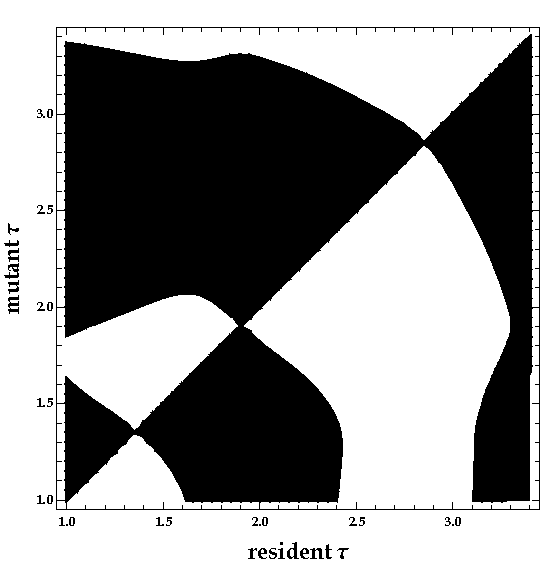
\includegraphics[width=\textwidth]{PIPbistability.pdf}}%
  \end{subfigure}\hspace{1cm}
  \begin{subfigure}[t]{0.3\textwidth}\hspace{0cm}
      \raisebox{-\height}{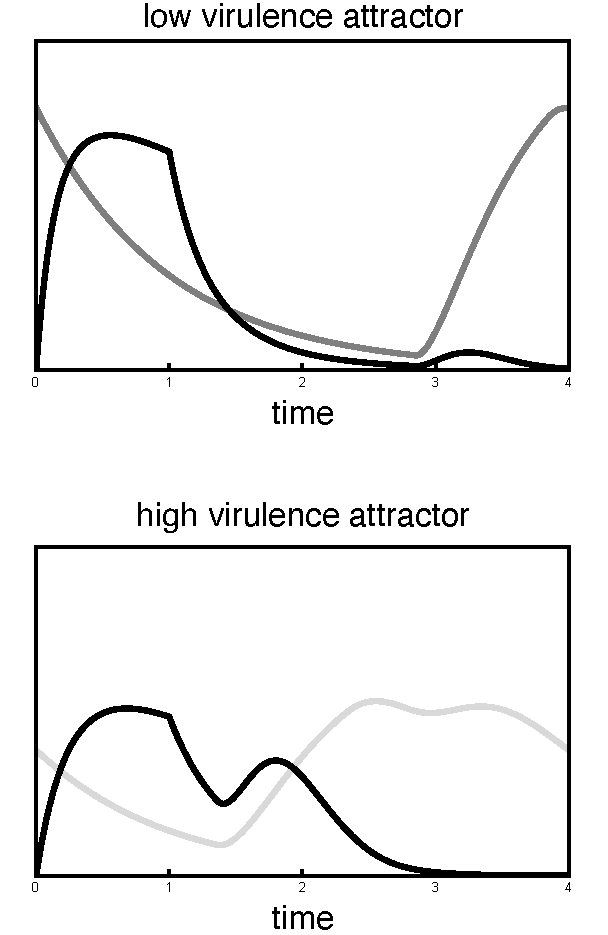
\includegraphics[width=\textwidth]{wsboth.pdf}}
  \end{subfigure}\hspace{1.5cm}
    \caption{\textbf{Seasonal host activity generates multiple parasite virulence attractors.} Left panel: Pairwise invasibility plot (PIP) shows the outcome of mutant invasion. Mutants possess an adaptive virulence ($\tau$) phenotype and invade in black regions while they possess a maladaptive virulence ($\tau$) phenotype and go extinct in white regions. The PIP shows two evolutionarily stable strategy (ESS) at $\tau \approx 2.85$ and $\tau \approx 1.35$ that are attractive and uninvasible. A repelloing and invasible evolutionary repellor lies between the two ESS at $\tau \approx 1.9$. Right panel: The low virulence attractor ($\tau \approx 2.85$) releases new parasites just prior to the end of the season and is thus monocyclic. The high virulence attractor ($\tau \approx 1.35$) is polycyclic and completes at least two generations of infections during the season (two generations of infection for the parameter values shown here). $T = 4, t_{l} = 1, \beta(\tau) = b (\tau+ 0.5)^{0.8}$, all other parameters in Table 1. }
\end{figure*}

\begin{figure*}[hb!]
  \centering
  \captionsetup[subfigure]{oneside,margin={0.1cm,0cm}}
    \begin{subfigure}[t]{0.45\textwidth}
      \centering
      \raisebox{-\height}{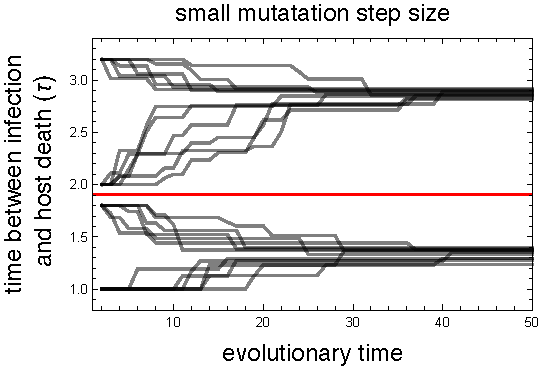
\includegraphics[width=\textwidth]{smutsims.pdf}}%
  \end{subfigure}\hspace{1cm}
  \begin{subfigure}[t]{0.45\textwidth}\hspace{0cm}
      \raisebox{-\height}{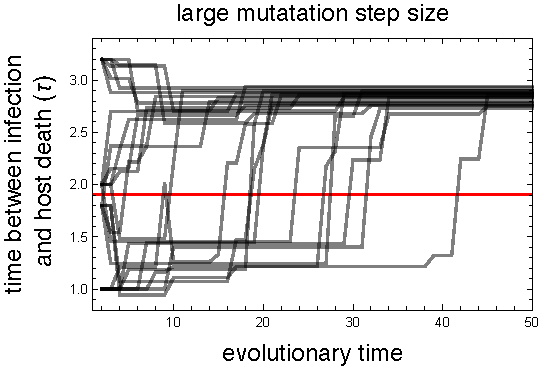
\includegraphics[width=\textwidth]{bmutsims.pdf}}
  \end{subfigure}\hspace{1.5cm}
    \caption{\textbf{Initial conditions determine which virulence attractor parasite populations evolve towards.} A repellor exists between the two attractors at moderate virulence around $\tau = 1.9$. If mutation step sizes are small, parasite populations with $\tau > 1.9$ evolve towards the low virulence, monocyclic attractor at $\tau \approx 2.85$ while parasite populations with $\tau < 1.9$ evolve towards the high virulence, polycyclic attractor at $\tau \approx 1.35$. If mutation step sizes are large, all parasite populations eventually reach the low virulence, monocyclic attractor as this is the global optimum for these parameters. Plots show 24 independent simulation analyses with high or low mutation step sizes. Six runs start at $\tau = 3.2$, $\tau = 2$, $\tau = 1.8$ and $\tau = 1$, respectively. Evolutionary time represents the number of mutants introduced into each system. In a random season after at least 1000 seasons have passed since the last mutant was introduced, the parasite population with the highest density is set as the "resident" population and a new mutant is introduced with a virulence phenotype drawn from a normal distribution whose mean is the virulence phenotype of the "resident" parasite population. When the mutation step size is small: $\tau_{m} = \tau_{r} + \mathcal{N}(0,0.1)$. When the mutation step size is large: $\tau_{m} = \tau_{r} + \mathcal{N}(0,0.5)$. Parameter values in this figure are identical to those in Figure 1. 
    }
\end{figure*}

\begin{figure*}[hb!]
  \centering
  \captionsetup[subfigure]{oneside,margin={0.1cm,0cm}}
    \begin{subfigure}[t]{0.45\textwidth}
      \centering
      \raisebox{-\height}{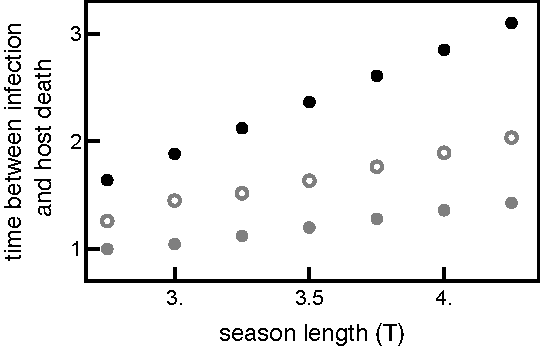
\includegraphics[width=\textwidth]{gmax_tt.pdf}}%
  \end{subfigure}\hspace{1cm}
  \begin{subfigure}[t]{0.45\textwidth}\hspace{0cm}
      \raisebox{-\height}{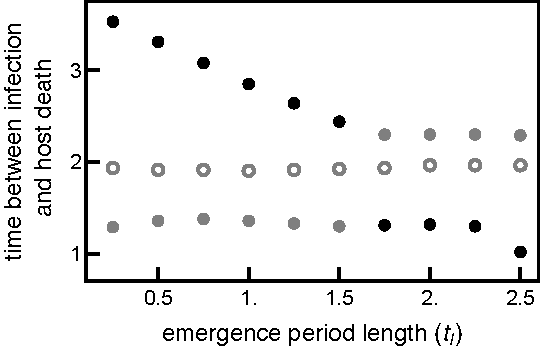
\includegraphics[width=\textwidth]{gmax_tl.pdf}}
  \end{subfigure}\hspace{1.5cm}
    \caption{\textbf{Host phenology impacts parasite virulence optimums. A.} Longer seasons select for lower virulence. \textbf{B.} Higher emergence variability selects for higher virulence for both high and low virulence attractor impact of changing emergence period length is nonlinear. The strength $t_{l}$ has on the respective attractors varies - increases in $t_{l}$ when $t_{l}< 1.75$ results in a large increase in virulence for the low virulence attractor but a small increase in virulence for the high virulence attractor while the opposite is true for $t_{l}> 1.75$. Black points mark global attractors, gray points mark local attractors and hollow points mark repellors. All other parameters are identical to those in Figure 1. 
    }
\end{figure*}

\begin{figure*}[hb!]
  \centering
  \captionsetup[subfigure]{oneside,margin={0.1cm,0cm}}
    \begin{subfigure}[t]{0.45\textwidth}
      \centering
      \raisebox{-\height}{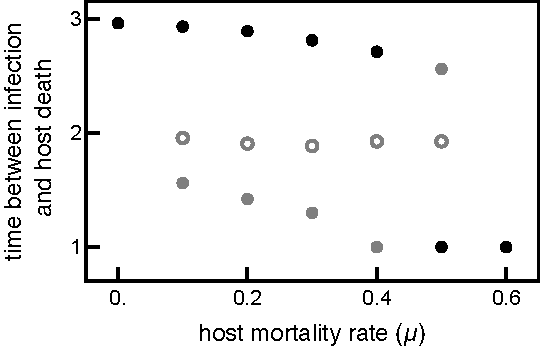
\includegraphics[width=\textwidth]{ga_mu.pdf}}%
  \end{subfigure}\hspace{1cm}
  \begin{subfigure}[t]{0.45\textwidth}\hspace{0cm}
      \raisebox{-\height}{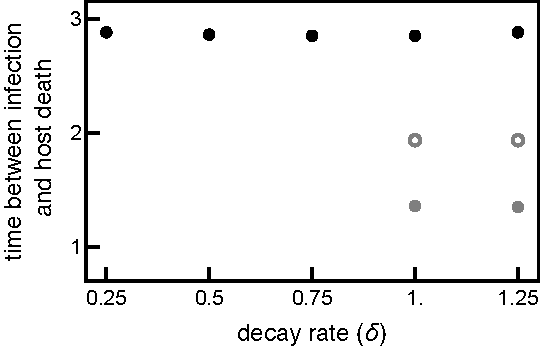
\includegraphics[width=\textwidth]{ga_delta.pdf}}
  \end{subfigure}\hspace{1cm}
    \begin{subfigure}[t]{0.45\textwidth}
      \centering
      \raisebox{-\height}{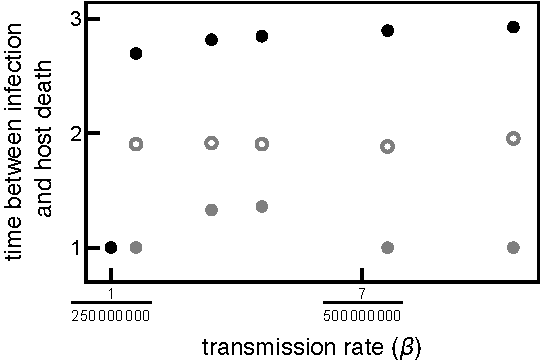
\includegraphics[width=\textwidth]{ga_beta.pdf}}%
  \end{subfigure}\hspace{1cm}
    \begin{subfigure}[t]{0.45\textwidth}
      \centering
      \raisebox{-\height}{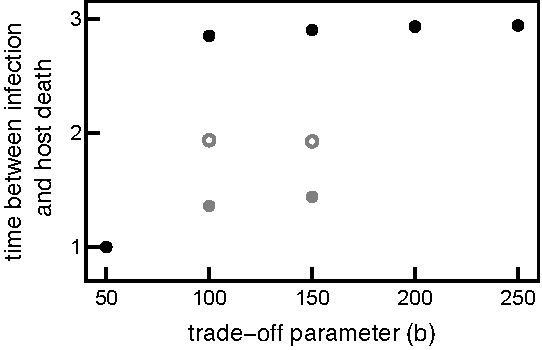
\includegraphics[width=\textwidth]{ga_b.pdf}}%
  \end{subfigure}\hspace{1.5cm}
    \caption{\textbf{Certain conditions can destroy bistability or switch the global optimum.} Parasite virulence attractors and repellors for changing: \textbf{A.} Host death rate, $\mu$ \textbf{B.} parasite decay rate, $\delta$ \textbf{C.} transmission rate, $\beta$ \textbf{D.} trade-off parameter, $b$. \textbf{A.} Low natural host mortality, $\mu$, drives high host densities and thus high early season incidence. High incidence early in the season selects for the low virulence, monocyclic strategy. High $\mu$ makes the high virulence, polycyclic attractor the global optimum as remaining in the host for long periods is risky. \textbf{B.} A low decay rate, $\delta$, drives high parasite densities and thus high early season incidence. High incidence early in the season selects for the low virulence, monocyclic attractor. \textbf{C.} A low transmission rate, $\beta$, pushes the timing of infections to later in the season. Late infections select for the high virulence, polycyclic strategy as there is less time between infection and the end of the season. Higher $\beta$ result in high early season incidence and thus drives both attractors towards lower virulence.  \textbf{D.} Low values of the trade-off parameter, $b$, result in low parasite density and thus slow incidence. High virulence is adaptive when incidence is slow as parasites have less time to release progeny before the end of the season. High values of $b$ result in high parasite density and thus high incidence early in the season. High early season incidence selects for the low virulence, monocyclic strategy. 
    $T = 4, t_{l} = 1$. When a parameter is not changing, its value is the same as in Table 1. 
    }
\end{figure*}

\begin{figure*}[hb!]
  \centering
  \captionsetup[subfigure]{oneside,margin={0.1cm,0cm}}
    \begin{subfigure}[t]{0.45\textwidth}
      \centering
      \raisebox{-\height}{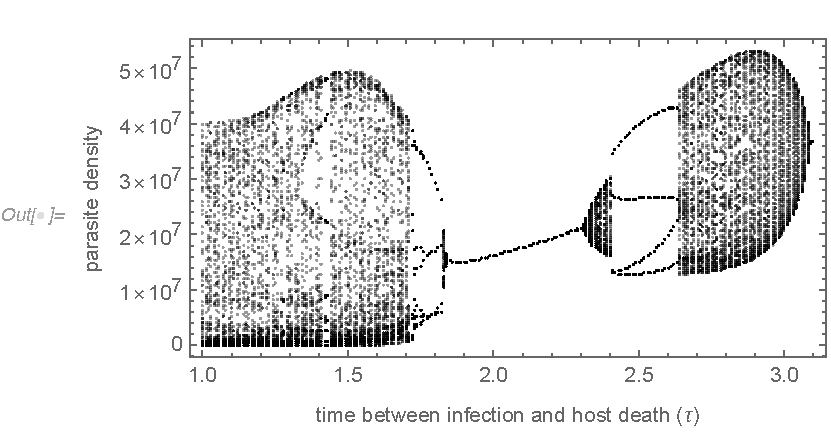
\includegraphics[width=\textwidth]{repellorbif.pdf}}%
  \end{subfigure}\hspace{1cm}
  \begin{subfigure}[t]{0.45\textwidth}\hspace{0cm}
      \raisebox{-\height}{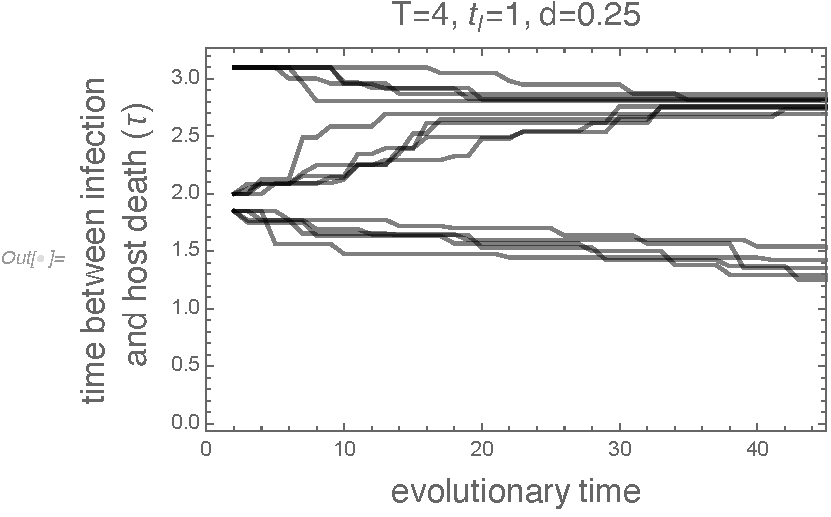
\includegraphics[width=\textwidth]{periodicsims.pdf}}
  \end{subfigure}\hspace{1.5cm}
    \caption{\textbf{Virulence evolution generates periodic dynamics when host populations carryover from one season to the next A.}
    Parasite density increases as the virulence phenotype approaches the time between infection and host death ($\tau$) that maximizes parasite fitness\cite{macdonald2021host}. Parasite populations can reach sufficiently high densities in some host phenological patterns to destabilize demographic dynamics resulting in a bifurcation that drives quasiperiodic parasite-host dynamics. The bifurcation diagram shows end of season parasite densities for parasites with different virulence phenotypes ($\tau$) for seasons 800-900 in a system where the host season is short ($T=4$) and hosts emerge synchronously ($t_{l}=1$). Moderate virulence parasites ($1.85<\tau<2.3$) reach a stable  equilibrium. The most fit parasites at high virulence ($\tau<1.85$) and low virulence ($\tau>2.3$) achieve densities that can disrupt dynamics and cause cycling. \textbf{B.} Periodic host-parasite dynamics do not qualitatively impact the evolutionary endpoints, \textit{i.e.} high and low virulence attractors are separated by a repellor despite periodic dynamics. The same simulation analysis with small mutation step size was used as described in Figure 2. All other parameters are the same as Table 1.
    }
\end{figure*}

%possible empirical system: Meloidogyne sp./Pasteuria penetrans - Meloidogyne are nematodes, and P. penetrans is an obligate-killer fungus that infects Meloidogyne. P. penetrans transmits by taking over nematode egg-laying machinery. All transmission occurs during the nematode plant host's growing season (http://entnemdept.ufl.edu/creatures/NEMATODE/Pasteuria_penetrans.html#:~:text=Pasteuria%20penetrans%20is%20an%20obligate,nematode%20host%20encounters%20the%20spore), (https://hal.archives-ouvertes.fr/hal-01402242/document)
%more parasites of nematodes here: https://www.apsnet.org/edcenter/disandpath/nematode/pdlessons/Pages/RootknotNematode.aspx

\section*{Discussion}
%summary paragraph
%parasites have two options: high virulence and try to get through multiple rounds of infection (risky) or low virulence and hope host doesn't die but decrease risk of decay for progeny
Host phenological patterns govern parasite virulence and drive the evolution of diverse strategies. Host phenology drives parasites either towards a high virulence strategy that completes multiple rounds of infection within the season (polycyclic) or towards a low virulence strategy that completes one round of infection within the season (monocyclic). Both the monocyclic and polycyclic strategies are evolutionarily stable attractors across phenological patterns. In between the two attractors is an evolutionary repellor. Which attractor a parasite population evolves towards is thus dependent on its starting virulence phenotype. The exact host phenological pattern also generates diversity by shifting the optima of both the high and low virulence strategies. While host seasonality did not drive evolutionary branching or the coexistence of diverse parasite strategies, these results predict that host seasonality could drive parasite diversity over geography. 

%results provide clues on evolutionary pressures and why either strategy can work. we further show how certain parameters make one strategy more competitive than the other (e.g. high host death rate favors polycyclic)
The result that host seasonality drives either high or low parasite virulence provides clues on the evolutionary drivers of monocylic and polycylic parasite strategies. The high virulence strategy is potentially risky for parasites as it relies on there being enough susceptible hosts when later generations of parasites are released. The low virulence strategy can be safer for parasites as it minimizes decay of new progeny in the environment, but only if the natural host mortality rate is low. Environmental conditions aside from host phenology also determine which strategy has a competitive edge. For example, the low virulence strategy is the  global optimum in environments that drive high parasite densities. High parasite densities result in high infection incidence early in the season which drives synchronous release of new parasites near the end of the season. Environments that favor low virulence thus simultaneously favor a monocylic parasite strategy. In contrast, the high virulence strategy is the global optimum in environments where remaining in the host is risky, such as when hosts have a high natural mortality rate. Environments where host life expectancy is short are thus predicted to drive the evolution of polycyclic parasites. 

%discuss previous work 
High parasite densities can drive cyclic host-parasite dynamics when host populations from one season reproduce and give rise to next season's host cohort. Cycling does not qualitatively alter the evolutionary result that either high virulence or low virulence evolves. These results are in line with previous results on a strictly monocyclic parasite\cite{} where high parasite density drives cycling and cycling does not alter evolutionary endpoints when compared to a model without cycling\cite{}. While we could not solve the current model analytically, previous work on the similar model suggested that cycles are driven by a Neimark-Sacker bifurcation which is likely the case in the current model. 

%discuss cycles, in fig. 5 it looks like high virulence parasite is at high risk of stochastic extinction when dynamics are cycling  
Cycling host-parasite dynamics could drive high virulence parasites extinct while maintaining low virulence parasite populations.
In the current model, when parasite populations evolve towards high virulence and drive cycling, those parasite populations at times have extremely low densities (Figure 5). In nature, these populations would be at high risk for stochastic extinction. In contrast, when parasite populations evolve towards low virulence and drive cycling, their densities remain high throughout the cycle. Thus in nature, high virulence parasites may be more likely to die out when cycling while low virulence parasites maintain safe densities that persist when cycling. 

%is there lit on similar parasites exhibiting opposite latency strategies? results could explain why similar geographic locations have very different parasite populations. maybe also look at lit on repellors to see if there are any pop gen refs on randomness of which mutation arises
%some wasps are more likely to be monocyclic at high altitudes (where seasons are shorter), could be that minimum latency period is too long to complete more than one parasite generation. in contrast, at lower altitudes similar/same(?) wasp species are more likely to be bicyclic
%propose experiments?
%The seasonal activity patterns of species with non-overlapping generations may have large impacts on the virulence strategies of the parasites they host. For example, ichneumonid parasitic wasp species are more likely to be monocylic at high altitudes and bicyclic or polycyclic at low altitudes. This observation has some similarities with our results. The model predicts that short seasons drive higher virulence for both evolutionary attractors. There are likely constraints on the minimum time between infection and progeny release. 

%extensions
%what happens when host populations are less limited? (I expect high virulence takes over) - discuss self-shading result here, if hosts reproduce more than once per season, high virulence might be a better strategy because self-shading maybe isn't as big of a problem
%what happens when some hosts survive between seasons, could this cause branching?
Several features of the current model can be altered to investigate more complex impacts of phenology on virulence evolution and parasite diversity. For example, relaxing the assumption that host populations reproduce once per season would likely favor the high virulence strategy. In the current model, the first generation of high virulence parasites in a season self-shades by killing too many hosts which results in few hosts remaining for the next generation of parasites to infect. Host reproduction throughout the season may reduce or eliminate the cost of self-shading and thus select for higher virulence. %Additionally, a host species that lives through several seasons could qualitatively change evolutionary endpoints by increasing selection for high virulence during the host activity period and low virulence after the host activity period. This extension could drive evolutionary branching in parasite virulence strategies. 
We will extend the current model to address these questions in future studies.

%caveats
The strict assumption that the parasites is an obligate host-killer can likely be relaxed without altering the result that phenology can drive the evolution of high or low virulence strategies. For example, many parasites reduce host fecundity or increase the host death rate upon progeny release. Longer latency periods are equivalent to lower virulence in this type of system as infected hosts have more time to reproduce and thus higher fitness. Relaxing the obligate-killer assumption would not likely alter our results qualitatively as the same evolutionary pressures would act on the timing of parasite release. That is, releasing new parasites quickly (high virulence) or releasing parasites near the end of the season (low virulence) would likely both be viable strategies. Many parasite-host systems conform to the assumptions of this model extension such as soil-borne plant pathogens, demicyclic rusts, post-harvest diseases, and many diseases systems infecting univoltine insects\cite{gaulin2007root,zehr1982control,crowell1934hosts,holuvsa2017pathogen}.


\bibliographystyle{unsrt}
\bibliography{biblio}

\end{document}

